\documentclass{article}

\usepackage[T2A]{fontenc}
\usepackage[utf8]{inputenc}
\usepackage[russian]{babel}

\usepackage[unicode, colorlinks, linkcolor=blue, citecolor=blue]{hyperref}

\usepackage{graphicx}
\graphicspath{{pictures/}}
\DeclareGraphicsExtensions{.pdf,.png,.jpg}

\begin{document}
\selectlanguage{russian}
	%----------------------------------Шапка------------------------------------
\begin{center}
	
\includegraphics[scale=0.25]{AU}\\
	{\Large\bfseries Санкт-Петербургский национальный исследовательский Академический университет имени Ж.И.~Алфёрова Российской академии наук}
\end{center}

\begin{center}
	{\large\textbf{Рабочий протокол и отчёт по лабораторной работе № 3}}\\
	Свиридов Фёдор, Александр Слободнюк
\end{center}

\begin{center}
	\rule{12cm}{0.4mm}\\
	\large\bfseries{<<Определение отношения теплоёмкостей $\gamma=\frac{C_p}{C_v}$ для воздуха методом Клемана - Дезорма>>}\\
	\rule{12cm}{0.4mm}
\end{center}
%-----------------------------------------------------------------------------
	\paragraph{Цель работы.} Определить показатель адиабаты воздуха
\paragraph{Задачи, решаемые при выполнении работы.}
\begin{enumerate}
	\item Измерить избыток давления в колбе в начале опыта
	\item Провести адиабатическое расширение газа
	\item Измерить избыток давления газа в колбе после изохорического нагревания
	\item Рассчитать адиабатический показатель 
	\item Проанализировать полученные результаты
\end{enumerate}
\paragraph{Объект исследования.} Проверка следствий из модели идеального газа.
\paragraph{Метод экспериментального исследования.} Измерения избытка давления в разных состояниях системы

\paragraph{Рабочие формулы и исходные данные.}\hypertarget{formuls}{}
\begin{figure}[htb]
	\centering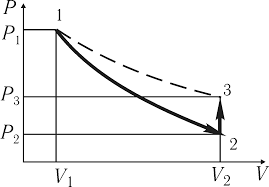
\includegraphics[scale=0.5]{plot}
	\caption{Зависимость давления газа от объема}
\end{figure}
\begin{equation}
	\gamma=\frac{\Delta P_1}{\Delta P_1 - \Delta P_3}
\end{equation}
где $\Delta P_1$ и $\Delta P_3$ избыток давления над атмосферным в состояниях 1 и 3, соответственно.

\paragraph{Результаты прямых измерений и их обработки.}

\begin{center}
\begin{tabular}{c|c|c}
	№& $\Delta P_1$, кПа & $\Delta P_3$, кПа \\
	\hline
	1& 13,9&3,3  \\
	2& 13,1&3,2  \\
	3&13,8 &2,8  \\
	4&13,8&2,9  \\
	5& 13,8&3,1  \\
	6& 13,5&2,8  \\
	7&14,3 &2,9  \\
	8& 13,6&3,1  \\
	9& 13,6&2,7  \\
	10& 13,3&2,7  \\
\end{tabular}
\end{center}

\paragraph{Расчет результатов косвенных измерений.}
	По рабочей формуле \hyperlink{formuls}{(1)} вычисляем показатель адиабаты для каждого опыта.
	
	Пример вычисления для первого случая:
	
	$$\gamma_1=\frac{13,9}{13,9-3,3}\approx1,3$$ 
	
		\begin{center}
		\begin{tabular}{c|c| c |c |c |c |c |c |c| c| c|  }
			№&1&2&3&4&5&6&7	&8&9&10\\
			\hline
			$\gamma$& 1,3 & 1,3& 1,2& 1,3& 1,3& 1,3& 1,2& 1,3& 1,2& 1,2
		\end{tabular}
	\end{center}
\paragraph{Погрешность измерений.}
$$<\gamma>=\frac{1}{N}\sum_{i=1}^{N}\gamma_i=1,26$$
$$\sigma=\sqrt{\frac{\sum_{i=1}^{N}(\gamma_i-<\gamma>)^2}{N-1}}=0,052$$
$$ \Delta\gamma=\frac{3\sigma}{\sqrt{N}}=0,05$$

 
\paragraph{Окончательные результаты.}
Показатель адиабаты воздуха:
$$\fbox{$\gamma=1,26\pm0,05$} $$
\paragraph{Выводы и анализ результатов.}
Мы вычислили показатель адиабаты воздуха. Полученные результаты согласуются с моделью идеального газа. Из теории следует, что  $\gamma=\frac{i+2}{i}$, считая что воздух состоит из двухатомных молекул, которые жёстко связаны между собой, то есть имеют 3 поступательные и 2 вращательные степени свободы, находим: $\gamma=\frac{5+2}{5}=1,4$.

Недостатком данного метода является то, что процессы быстрого расширения газа в ходе лабораторной работы не являются чисто адиабатическими, так как существует теплообмен со стенками сосуда, а также то, что рассматриваемый газ не является идеальным. Кроме этого данный метод имеет существенный недостаток в том, что практически невозможно добиться того, чтобы длительность открывания клапана в точности совпадала бы со временем его адиабатического расширения. Таким образом, в ходе эксперимента у нас получались то завышенные , то заниженные показатели $\Delta P_3$. Данные методические ошибки можно устранить, например, за счёт учёта времени расширения и количества подведённого за это время тепла.

\end{document}
